\documentclass[9pt]{beamer}
\usetheme{Warsaw}
\usefonttheme[onlymath]{serif}

\usepackage[utf8]{inputenc}
%\usepackage[polish]{babel}
\usepackage[T1]{fontenc}
\usepackage{comment}
\usepackage{setspace}
\usepackage{amsmath}
\usepackage{dcolumn}
\usepackage{siunitx}
\usepackage{tabularx}
\usepackage{graphicx}
\usepackage{changepage}
\usepackage{svg}
\usepackage[backend=biber,style=numeric,sorting=nyt,language=polish]{biblatex} % Konfiguracja biblatex
\addbibresource{references.bib} % Link the .bib file

\sisetup{
    table-number-alignment = center, % Align numbers at the decimal point
    table-format = +1.6e3,           % Specify number format: 1 digit before, 6 after decimal, and 1 exponent
    tight-spacing = true,           % Remove extra spacing around numbers
    scientific-notation = true,
}

\newcolumntype{M}{>{\centering\arraybackslash\math}p{2cm}}

\linespread{1}

%\newcommand\eqozn{\stackrel{\mathclap{\normalfont\mbox{\normalfont\tiny ozn}}}{=}}
\newcommand\eqozn{\mathrel{\overset{\makebox[0pt]{\mbox{\scriptsize ozn}}}{=}}}

\title{Projekt 2, Zadanie 36}
\author{Wiktor Murawski, 333255, grupa 3, środa 12:15}
\date{}

\begin{document}

\begin{frame}
    %\frametitle{\insertauthor,\space\inserttitle}
    \begin{spacing}{1.75}
    \begin{center}
        \inserttitle\par
        \insertauthor
    \end{center}
    \vspace{2em}
    Metoda Adamsa-Bashfortha rzędu 4-go dla liniowych równań różniczkowych pierwszego i drugiego rzędu. Wartości początkowe $y_1$, $y_2$, $y_3$ obliczane metodą Rungego-Kutty rzędu 4-go (wzór Ralstona). 
    \end{spacing}
\end{frame}

\section{Wprowadzenie}
\begin{frame}{Równanie różniczkowe pierwszego rzędu}
    Dane jest równanie różniczkowe liniowe pierwszego rzędu oraz warunek początkowy:
    \begin{equation*}
        \label{eq1}
        a_1(x)y' + a_0(x)y = b(x), \qquad y(x_0) = y_0
    \end{equation*}
    %na przedziale $\begin{bmatrix} x_0, x_N \end{bmatrix}$ 

    \hspace{2cm}
    
    Przekształcając równanie otrzymujemy
    \begin{equation*}
        y' = f(x,y) = \frac{b(x) - a_0(x)y}{a_1(x)}
    \end{equation*}
    
\end{frame}

\begin{frame}{Równanie różniczkowe drugiego rzędu}
    Dane jest równanie różniczkowe liniowe drugiego rzędu oraz warunki początkowe:
    \begin{equation*}
        \label{eq2}
        a_2(x)y'' + a_1(x)y' + a_0(x)y = b(x), \qquad \begin{matrix}y(x_0) = y_0 \\ y'(x_0) = y'_0\end{matrix}
    \end{equation*}
    %na przedziale $\begin{bmatrix} x_0, x_N \end{bmatrix}$

    Sprowadzamy równanie do układu równań różniczkowych liniowych stopnia pierwszego: 
    \[ Y' = F(x,Y), \] gdzie
    \begin{equation*}
        Y = \begin{bmatrix} y \\ y' \end{bmatrix} \eqozn \begin{bmatrix} y_1 \\ y_2 \end{bmatrix} \qquad\qquad Y' = \begin{bmatrix} y_1' \\ y_2' \end{bmatrix}
    \end{equation*}

    Przekształacając równanie otrzymujemy
    \begin{equation*}
        Y' = F(x,Y) = \begin{bmatrix} y_2 \\ \dfrac{1}{a_2(x)}(b(x) - a_0y_1 - a_1y_2) \end{bmatrix}
    \end{equation*}
    
\end{frame}

\section{Metoda Rungego-Kutty (Ralston)}
\begin{frame}{Jawne metody Rungego-Kutty 4-go rzędu}
    Mając wartość $Y_n$, jawne metody Rungego-Kutty rzędu czwartego pozwalają na wyznaczenie wartości $Y_{n+1}$ następująco:
    $$ \begin{aligned}
        K_1 &= hF(x_n, Y_n) \\
        K_2 &= hF(x_n + a_2h, Y_n + b_{21}K_1) \\
        K_3 &= hF(x_n + a_3h, Y_n + b_{31}K_1 + b_{32}K_2) \\
        K_4 &= hF(x_n + a_4h, Y_n + b_{41}K_1 + b_{42}K_2 + b_{43}K_3) \\
        Y_{n+1} - Y_n &= c_1K_1 + c_2K_2 + c_3K_3 + c_4K_4
    \end{aligned} $$
    Współczynniki $a_i, b_{ij},c_i$ przedstawione w tablicy Butchera:
    $$\begin{array}{c|cccc}
    0 & 0 & 0 & 0 & 0 \\
    a_2 & b_{21} & 0 & 0 & 0 \\
    a_3 & b_{31} & b_{32} & 0 & 0 \\
    a_4 & b_{41} & b_{42} & b_{43} & 0 \\ \hline
    & c_1 & c_2 & c_3 & c_4
    \end{array}$$
\end{frame}

\begin{frame}{Ogólne wzory na współczynniki}
    \newcommand{\1}{\alpha}
    \newcommand{\2}{\beta}

    \small
    
    Współczynniki $a_i, b_{ij},c_i$ tworzą rodzinę dwuparametrową zależną od parametrów $\1$ i $\2$ gdzie $\1 \neq 0, \2 \neq 0, \1 \neq 1, \2 \neq 1, \1 \neq \2$.

    \normalsize
    \renewcommand{\arraystretch}{2.5}
    \begin{adjustwidth}{-2.5em}{-3em}
    \scalebox{0.55}{$
    \begin{array}{c|ccccc}
    0 & 0 & 0 & 0 & 0  \\
    \1 & \1 & 0 & 0 & 0  \\
    \2 & \2 - \dfrac{\2(\2-\1)}{2\1(1-2\1)} & \dfrac{\2(\2-\1)}{2\1(1-2\1)} & 0 & 0  \\
    1 & 
1 - \dfrac{(1-\1)(\2(\1+\2-1-(2\2-1)^2) + 2\1(1-2\1)(1-\2))}{2\1\2(\2-\1)(6\1\2-4(\1+\2)+3)}
    
% \dfrac
% {12\1^2\2^2 + 12\1^2\2 - 4\1^2 + 12\1\2^2 - 15\1\2 + 6\1 - 4\2^2 + 5\2 - 2}
% {2\1\2(4\1 + 4\2 - 6\1\2 - 3)}
& \dfrac{(1-\1)(\1+\2-1-(2\2-1)^2)}{2\1(\2-\1)(6\1\2-4(\1+\2)+3)} & \dfrac{(1-2\1)(1-\1)(1-\2)}{\2(\2-\1)(6\1\2-4(\1+\2)+3)} & 0  \\ \hline
      & \dfrac{1}{2}-\dfrac{1-2(\1+\2)}{12\1\2} & \dfrac{2\2 - 1}{12\1(\2-\1)(1-\1)} & \dfrac{1 - 2\1}{12\2(\2-\1)(1-\2)} & \dfrac{1}{2}+\dfrac{2(\1+\2)-3}{12(1-\1)(1-\2)}
    \end{array}
    $}
    \end{adjustwidth}

    \vspace{0.1cm}

    \small
    
    Dla parametrów $\alpha = \frac{2}{5} \text{ i } \beta = \frac{7}{8} - \frac{3\sqrt5}{16}$ otrzymujemy ograniczenie górne na $E$, gdzie:
    \[ y(x_{n+1}) = y_{n+1} + Eh^5 \]
    \[ |E| < 5.46\cdot10^{-2}ML^4 \]
    gdzie, dla pewnego obszaru $B(x,y)$ zawierającego $(x_n,y_n)$, zachodzi
    $$|f(x,y)| \leq M \qquad\qquad \dfrac{\partial^{i+j}f}{\partial x^i\partial y^j} < \dfrac{L^{i+j}}{M^{j-1}} $$
    
\end{frame}

\begin{frame}{Tabela Butchera (wartości dokładne)}
    % Wyznaczone wartości współczynników dla parametrów minimalizujących ograniczenie górne błędu ($\alpha = \frac{2}{5} \text{ i } \beta = \frac{7}{8} - \frac{3\sqrt5}{16}$). Dla tych $\alpha$ i $\beta$:

    % \vspace{16pt}
    \renewcommand{\arraystretch}{2.5}
    \scalebox{0.80}{$
    \begin{array}{c|cccc}
    0 & 0 & 0 & 0 & 0 \\
    \dfrac{2}{5}            & \dfrac{2}{5}                          & 0                                     & 0                                                 & 0 \\
    \dfrac{14-3\sqrt5}{16}  & \dfrac{-2\,889 + 1\,428\sqrt5}{1\,024}   & \dfrac{3\,785 - 1\,620\sqrt5}{1\,024}    & 0                                                 & 0 \\
    1                       & \dfrac{-3\,365 + 2\,094\sqrt5}{6\,040}   & \dfrac{-975 - 3\,046\sqrt5}{2\,552}     & \dfrac{467\,040 + 203\,968\sqrt5}{240\,845}          & 0 \\ \hline
                            & \dfrac{263 + 24\sqrt5}{1\,812}         & \dfrac{125 - 1\,000\sqrt5}{3\,828}       & \dfrac{3\,426\,304 + 1\,661\,952\sqrt5}{5\,924\,787}    & \dfrac{30 - 4\sqrt5}{123}
    \end{array}
    $}
\end{frame}

\begin{frame}{Tabela Butchera (wartości przybliżone)}
    \renewcommand{\arraystretch}{1.5} % Adjust row spacing for better readability
    % \scalebox{1}{$
    % \begin{array}{c|ccccc}
    % 0 & 0 & 0 & 0 & 0  \\
    % 0.4 & 0.4 & 0 & 0 & 0  \\
    % 0.45573725 & 0.29697761 & 0.15875964 & 0 & 0  \\
    % 1 & 0.21810040 & -3.05096516 & 3.83286476 & 0  \\ \hline
    %   & 0.17476028 & -0.55148066 & 1.20553560 & 0.17118478
    % \end{array}
    % $}
    \scalebox{1}{$
    \begin{array}{c|ccccc}
    0 & 0 & 0 & 0 & 0  \\
    0.4 & 0.4 & 0 & 0 & 0  \\
    0.45573725 & 0.29697761 & 0.15875964 & 0 & 0  \\
    1 & 0.21810039 & -3.05096515 & 3.83286476 & 0  \\ \hline
      & 0.17476028 & -0.55148066 & 1.20553560 & 0.17118478
    \end{array}
    $}
\end{frame}

\section{Metoda Adamsa-Bashfortha}
\begin{frame}{Metoda Adamsa-Bashfortha}
    Metoda Adamsa-Bashfortha rzędu czwartego jest metodą wielokrokową opartą na 4 węzłach: $x_n, x_{n-1}, x_{n-2}, x_{n-3}$.
    $Y_{n+1}$ obliczane jest następująco:
    \[Y_{n+1} = Y_n + h\sum\limits^{3}_{i=0}\alpha_iF(Y_{n-i})\]
    Z faktu, że $Y' = F(x,Y)$, otrzymujemy:
    \[ \int_{x_n}^{x_{n+1}}Y'(x)dx = \int_{x_n}^{x_{n+1}}F(Y(x))dx \]
    \[ Y(x_{n+1}) = Y(x_n) + \int_{x_n}^{x_{n+1}}F(Y(x))dx \]
    Chcemy dobrać współczynniki $\alpha_i$ tak, aby metoda dawała najlepsze przybliżenie całki w powyższym wyrażeniu.
\end{frame}

\begin{frame}{Współczynniki metody Adamsa-Bashfortha}
    Chcemy, aby kwadratura 
    \[ h\sum\limits^{3}_{i=0}\alpha_iF(Y_{n-i}) \approx 
    \int_{x_n}^{x_{n+1}}F(Y(x))dx \]
    była dokładna dla wielomianów stopnia $\leq 3$.\\

    Wyznaczone współczynniki mają następujące wartości:
    \[ \alpha_0 = \dfrac{55}{24} \qquad \alpha_1 = -\dfrac{59}{24} \qquad \alpha_2 = \dfrac{37}{24} \qquad \alpha_3 = -\dfrac{9}{24}\]

    Ostatecznie otrzymujemy:
    \[ Y_{n+1} = Y_n + h \left( \dfrac{55}{24}F(Y_n) - \dfrac{59}{24}F(Y_{n-1}) + \dfrac{37}{24}F(Y_{n-2}) - \dfrac{9}{24}F(Y_{n-3})  \right) \]
\end{frame}

\section{Testy}
\begin{frame}{Testy poprawności}
    $$y' = 4x^3, \qquad y(0) = 0, \qquad x\in[0,10]$$
    \centering
    Rozwiązanie: $y = x^4$
    \begin{table}[]
    	\makebox[\linewidth]{
    		\begin{tabular}{|l|l|S|}
    			% \hline & & \\[-1em]
                \hline & & \\ [-10pt]
    			$i$ & {$h = 2^{-i}$} & {Błąd globalny} \\ [-1pt] \hline & & \\ [-10pt]
    			% \hline & &\\[-1em]
    			%---------------------------------------------------------------------------				
0  & $ 1.0          $ & 1.421085e-14 \\ [-1pt] \hline & & \\ [-10pt]
1  & $ 0.5          $ & 8.881784e-16 \\ [-1pt] \hline & & \\ [-10pt]
2  & $ 0.25         $ & 5.551115e-17 \\ [-1pt] \hline & & \\ [-10pt]
3  & $ 0.125        $ & 3.469447e-18 \\ [-1pt] \hline & & \\ [-10pt]
4  & $ 0.0625       $ & 2.168404e-19 \\ [-1pt] \hline & & \\ [-10pt]
5  & $ 0.03125      $ & 1.355253e-20 \\ [-1pt] \hline & & \\ [-10pt]
6  & $ 0.015625     $ & 8.470329e-22 \\ [-1pt] \hline & & \\ [-10pt]
7  & $ 0.0078125    $ & 5.293956e-23 \\ [-1pt] \hline & & \\ [-10pt]
8  & $ 0.00390625   $ & 3.308722e-24 \\ [-1pt] \hline & & \\ [-10pt]
9  & $ 0.001953125  $ & 2.067952e-25 \\ [-1pt] \hline & & \\ [-10pt]
10 & $ 0.0009765625 $ & 1.292470e-26 \\ \hline % & & \\ [-10pt]
    			%---------------------------------------------------------------------------
            \end{tabular}
    	}
    \end{table}
\end{frame}

\begin{frame}{Testy poprawności}
    $$y'' = 12x^2, \qquad y(0) = 0, \quad y'(0) = 0, \qquad x\in[0,10]$$
    \centering
    Rozwiązanie: $y = x^4$
    \begin{table}[]
    	\makebox[\linewidth]{
    		\begin{tabular}{|l|l|S|}
    			% \hline & & \\[-1em]
                \hline & & \\ [-10pt]
    			$i$ & {$h = 2^{-i}$} & {Błąd globalny} \\ [-1pt] \hline & & \\ [-10pt]
    			% \hline & &\\[-1em]
    			%---------------------------------------------------------------------------				
0  & $ 1.0          $ & 1.421085e-13 \\ [-1pt] \hline & & \\ [-10pt]
1  & $ 0.5          $ & 8.881784e-15 \\ [-1pt] \hline & & \\ [-10pt]
2  & $ 0.25         $ & 5.551115e-16 \\ [-1pt] \hline & & \\ [-10pt]
3  & $ 0.125        $ & 3.469447e-17 \\ [-1pt] \hline & & \\ [-10pt]
4  & $ 0.0625       $ & 2.168404e-18 \\ [-1pt] \hline & & \\ [-10pt]
5  & $ 0.03125      $ & 1.355253e-19 \\ [-1pt] \hline & & \\ [-10pt]
6  & $ 0.015625     $ & 8.470329e-21 \\ [-1pt] \hline & & \\ [-10pt]
7  & $ 0.0078125    $ & 5.293956e-22 \\ [-1pt] \hline & & \\ [-10pt]
8  & $ 0.00390625   $ & 3.308722e-23 \\ [-1pt] \hline & & \\ [-10pt]
9  & $ 0.001953125  $ & 2.067952e-24 \\ [-1pt] \hline & & \\ [-10pt]
10 & $ 0.0009765625 $ & 1.292470e-25 \\ \hline % & & \\ [-10pt]
    			%---------------------------------------------------------------------------
            \end{tabular}
    	}
    \end{table}
\end{frame}

\begin{frame}{Testy poprawności}
    $$y' = 5x^4, \qquad y(0) = 0, \qquad x\in[0,10]$$
    \centering
    Rozwiązanie: $y = x^5$
    \begin{table}[]
    	\makebox[\linewidth]{
    		\begin{tabular}{|l|l|S|}
    			% \hline & & \\[-1em]
                \hline & & \\ [-10pt]
    			$i$ & {$h = 2^{-i}$} & {Błąd globalny} \\ [-1pt] \hline & & \\ [-10pt]
    			% \hline & &\\[-1em]
    			%---------------------------------------------------------------------------				
0  & $ 1.0           $ & 2.926973e+02 \\ [-1pt] \hline & & \\ [-10pt]
1  & $ 0.5           $ & 2.221971e+01 \\ [-1pt] \hline & & \\ [-10pt]
2  & $ 0.25          $ & 1.511423e+00 \\ [-1pt] \hline & & \\ [-10pt]
3  & $ 0.125         $ & 9.829805e-02 \\ [-1pt] \hline & & \\ [-10pt]
4  & $ 0.0625        $ & 6.263444e-03 \\ [-1pt] \hline & & \\ [-10pt]
5  & $ 0.03125       $ & 3.952096e-04 \\ [-1pt] \hline & & \\ [-10pt]
6  & $ 0.015625      $ & 2.481748e-05 \\ [-1pt] \hline & & \\ [-10pt]
7  & $ 0.0078125     $ & 1.555003e-06 \\ [-1pt] \hline & & \\ [-10pt]
8  & $ 0.00390625    $ & 9.727955e-08 \\ [-1pt] \hline & & \\ [-10pt]
9  & $ 0.001953125   $ & 6.097252e-09 \\ [-1pt] \hline & & \\ [-10pt]
10 & $ 0.0009765625  $ & 3.565219e-10 \\ \hline % & & \\ [-10pt]
    			%---------------------------------------------------------------------------
            \end{tabular}
    	}
    \end{table}
\end{frame}

\begin{frame}{Testy poprawności}
    $$y'' = 20x^3, \qquad y(0) = 0, \quad y'(0) = 0, \qquad x\in[0,10]$$
    \centering
    Rozwiązanie: $y = x^5$
    \begin{table}[]
    	\makebox[\linewidth]{
    		\begin{tabular}{|l|l|S|}
    			% \hline & & \\[-1em]
                \hline & & \\ [-10pt]
    			$i$ & {$h = 2^{-i}$} & {Błąd globalny} \\ [-1pt] \hline & & \\ [-10pt]
    			% \hline & &\\[-1em]
    			%---------------------------------------------------------------------------				
0  & $1.0           $ & 2.933776e+02 \\ [-1pt] \hline & & \\ [-10pt]
1  & $0.5           $ & 2.224097e+01 \\ [-1pt] \hline & & \\ [-10pt]
2  & $0.25          $ & 1.512087e+00 \\ [-1pt] \hline & & \\ [-10pt]
3  & $0.125         $ & 9.831881e-02 \\ [-1pt] \hline & & \\ [-10pt]
4  & $0.0625        $ & 6.264093e-03 \\ [-1pt] \hline & & \\ [-10pt]
5  & $0.03125       $ & 3.952298e-04 \\ [-1pt] \hline & & \\ [-10pt]
6  & $0.015625      $ & 2.481812e-05 \\ [-1pt] \hline & & \\ [-10pt]
7  & $0.0078125     $ & 1.555018e-06 \\ [-1pt] \hline & & \\ [-10pt]
8  & $0.00390625    $ & 9.727955e-08 \\ [-1pt] \hline & & \\ [-10pt]
9  & $0.001953125   $ & 6.097252e-09 \\ [-1pt] \hline & & \\ [-10pt]
10 & $0.0009765625  $ & 3.565219e-10 \\ \hline % & & \\ [-10pt]
    			%---------------------------------------------------------------------------
            \end{tabular}
    	}
    \end{table}
\end{frame}

\begin{frame}
	\frametitle{Testy numeryczne}
	\begin{spacing}{1.25}
        Zaimplementowana metoda Adamsa-Bashfortha jest rzędu czwartego, zatem błąd globalny 
        $$ E = \max \limits_{0\leq k \leq N} |y(x_k) - y_k| $$
        powinien zmieniać się proporcjonalnie do $h^4$. Przykładowo, dwukrotne zmniejszenie $h$ powinno spowodować szesnastokrotne zmniejszenie wartości błędu globalnego.
	\end{spacing}
\end{frame}

\begin{frame}{Testy numeryczne}
\vspace{-11pt}
    $$y'' - 2y' + 2y = 0, \qquad y(0) = 1, \quad y'(0) = 0, \qquad x\in[0,10]$$
    \centering
    Rozwiązanie: $y = e^x(\cos(x) - \sin(x))$
    \begin{table}[]
    	\makebox[\linewidth]{
    		\begin{tabular}{|l|l|S|c|}
    			% \hline & & \\[-1em]
                \hline & & & \\ [-10pt]
    			$i$ & {$h = 2^{-i}$} & {Błąd globalny} & Zmiana błędu \\ [-1pt] \hline & & & \\ [-10pt]
    			% \hline & &\\[-1em]
                %------------------
0  & $ 1.0             $ & 8.090118e+04 & --- \\ [-1pt]      \hline & & & \\ [-10pt]
1  & $ 0.5             $ & 8.386933e+03 & $ 9.646  $ \\ [-1pt]    \hline & & & \\ [-10pt]
2  & $ 0.25            $ & 3.662088e+02 & $ 22.902 $  \\ [-1pt]   \hline & & & \\ [-10pt]
3  & $ 0.125           $ & 4.481169e+01 & $ 8.172  $ \\ [-1pt]    \hline & & & \\ [-10pt]
4  & $ 0.0625          $ & 3.849399e+00 & $ 11.641 $  \\ [-1pt]   \hline & & & \\ [-10pt]
5  & $ 0.03125         $ & 2.780551e-01 & $ 13.844 $  \\ [-1pt]   \hline & & & \\ [-10pt]
6  & $ 0.015625        $ & 1.862380e-02 & $ 14.930 $  \\ [-1pt]   \hline & & & \\ [-10pt]
7  & $ 0.0078125       $ & 1.204076e-03 & $ 15.467 $  \\ [-1pt]   \hline & & & \\ [-10pt]
8  & $ 0.00390625      $ & 7.652592e-05 & $ 15.734 $  \\ [-1pt]   \hline & & & \\ [-10pt]
9  & $ 0.001953125     $ & 4.822753e-06 & $ 15.868 $  \\ [-1pt]   \hline & & & \\ [-10pt]
10 & $ 0.0009765625    $ & 3.027453e-07 & $ 15.930 $  \\ [-1pt]   \hline & & & \\ [-10pt]
11 & $ 0.00048828125   $ & 1.870649e-08 & $ 16.184 $  \\ [-1pt]   \hline & & & \\ [-10pt]
12 & $ 0.000244140625  $ & 1.072294e-09 & $ 17.445 $  \\ [-1pt]   \hline & & & \\ [-10pt]
13 & $ 0.0001220703125 $ & 5.074980e-10 & $ 2.113  $ \\ \hline % & & \\ [-10pt]
    			%------------------
            \end{tabular}
    	}
    \end{table}
\end{frame}

\begin{frame}{Testy numeryczne - porównanie do ode45}
\vspace{-2pt}
\centering
    $y'' + xy' + x^2y = x^3, \qquad y(0) = 0, \quad y'(0) = 0, \qquad x\in[0,3]$ \\
    \vspace{0pt}
    \centering
    \small
    Za dokładne wartości $y$ przyjęto rozwiązanie uzyskane przez użycie funkcji \texttt{ode45} środowiska MATLAB z ustawieniami \texttt{RelTol=1e-12} oraz \texttt{AbsTol=1e-12}.
    \vspace{-2pt}
    \normalsize
    \begin{table}[]
    	\makebox[\linewidth]{
    		\begin{tabular}{|l|l|S|c|}
    			% \hline & & \\[-1em]
                \hline & & & \\ [-10pt]
    			$i$ & {$h = 2^{-i}$} & {Błąd globalny} & Zmiana błędu \\ [-1pt] \hline & & & \\ [-10pt]
    			% \hline & &\\[-1em]
                %------------------
0  & $ 1.0             $ & 1.607416e-01 & --- \\ [-1pt]      \hline & & & \\ [-10pt]
1  & $ 0.5             $ & 6.927388e-01 & $ 0.232  $\\ [-1pt]    \hline & & & \\ [-10pt]
2  & $ 0.25            $ & 1.772034e-02 & $ 39.093 $ \\ [-1pt]   \hline & & & \\ [-10pt]
3  & $ 0.125           $ & 1.231859e-03 & $ 14.385 $ \\ [-1pt]    \hline & & & \\ [-10pt]
4  & $ 0.0625          $ & 7.846671e-05 & $ 15.699 $ \\ [-1pt]   \hline & & & \\ [-10pt]
5  & $ 0.03125         $ & 4.937812e-06 & $ 15.891 $ \\ [-1pt]   \hline & & & \\ [-10pt]
6  & $ 0.015625        $ & 3.085769e-07 & $ 16.002 $ \\ [-1pt]   \hline & & & \\ [-10pt]
7  & $ 0.0078125       $ & 1.927596e-08 & $ 16.008 $ \\ [-1pt]   \hline & & & \\ [-10pt]
8  & $ 0.00390625      $ & 1.204157e-09 & $ 16.008 $ \\ [-1pt]   \hline & & & \\ [-10pt]
9  & $ 0.001953125     $ & 7.514256e-11 & $ 16.025 $ \\ [-1pt]   \hline & & & \\ [-10pt]
10 & $ 0.0009765625    $ & 4.589662e-12 & $ 16.372 $ \\ [-1pt]   \hline & & & \\ [-10pt]
11 & $ 0.00048828125   $ & 4.662937e-13 & $ 9.843  $\\ [-1pt]   \hline & & & \\ [-10pt]
12 & $ 0.000244140625  $ & 6.226131e-13 & $ 0.749  $\\ [-1pt]   \hline & & & \\ [-10pt]
13 & $ 0.0001220703125 $ & 6.359357e-13 & $ 0.979  $\\ \hline % & & \\ [-10pt]
    			%------------------
            \end{tabular}
    	}
    \end{table}
\end{frame}

\begin{frame}{Wykres zależności błędu globalnego od wartości kroku}
    \centering
    $y'' = 20x^3, \qquad y(0) = 0, \quad y'(0) = 0, \qquad x\in[0,100]$
    %\vspace{-3pt}
    \begin{figure}
        \centering
        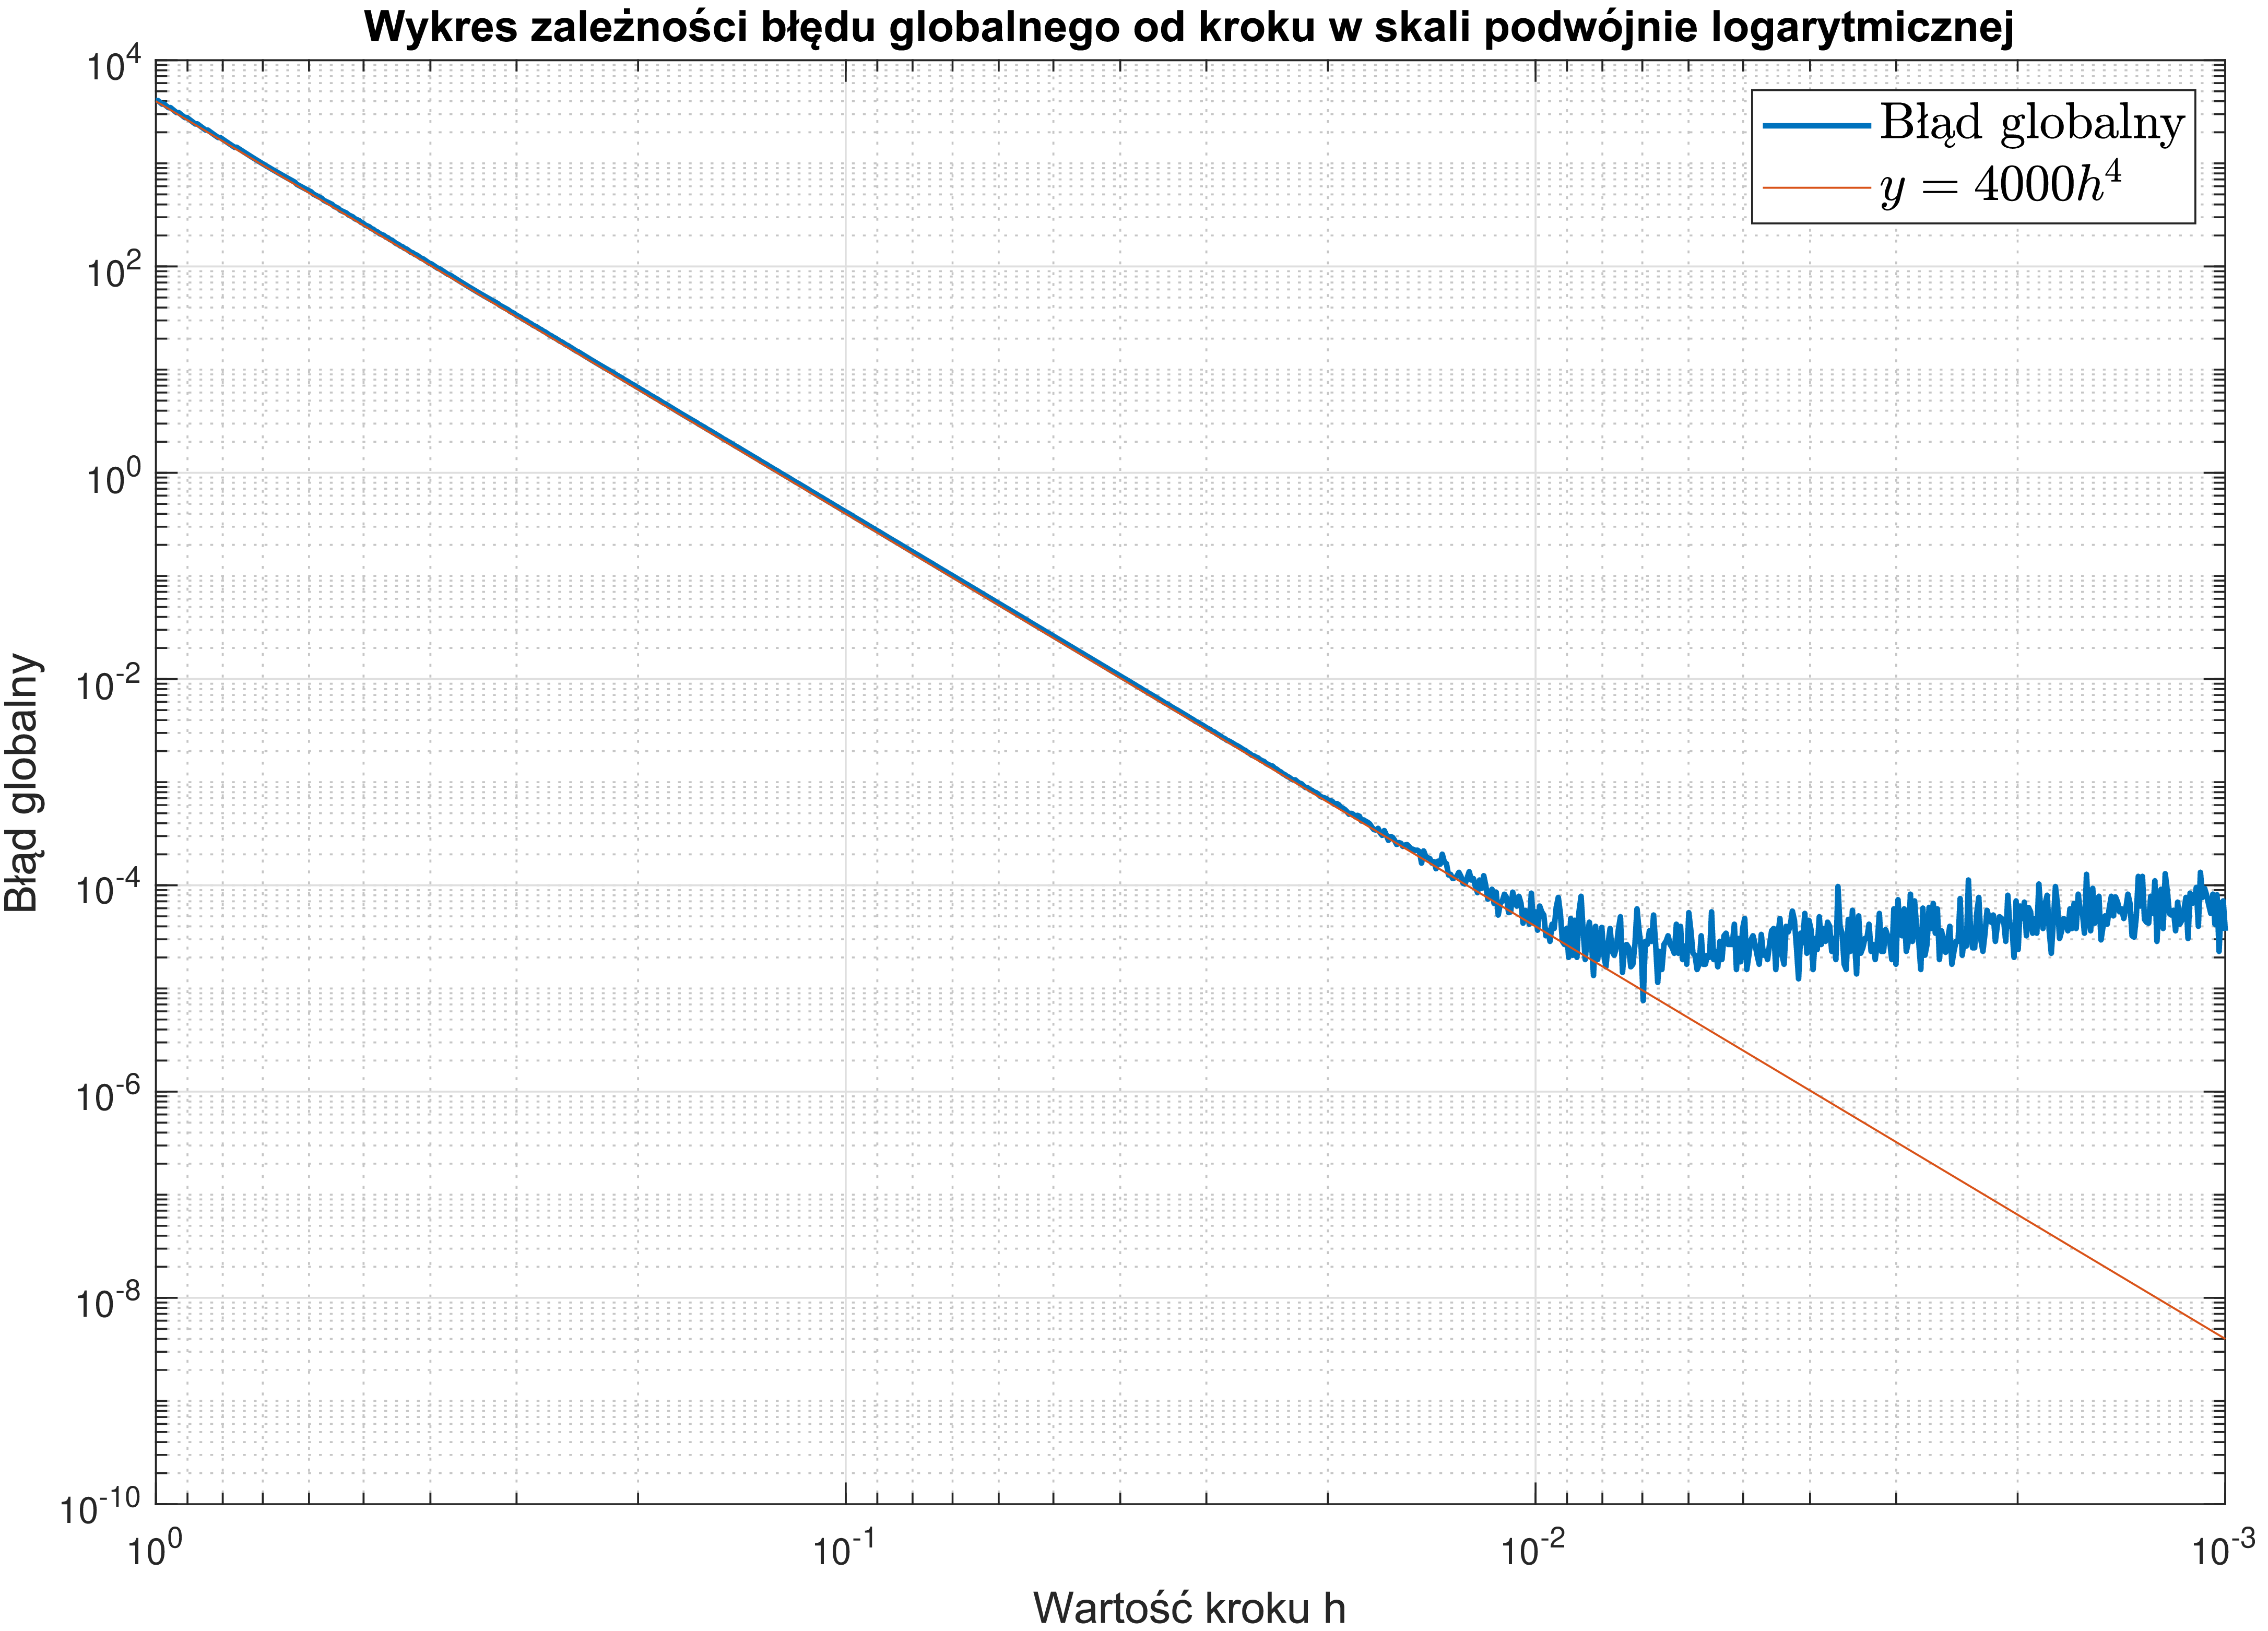
\includegraphics[width=0.9\linewidth]{smaller.png}
    \end{figure}
    
\end{frame}

\begin{frame}
	\frametitle{Źródła}
    \nocite{*}
    \printbibliography
\end{frame}

\end{document}